\chapter{Proposed solution}
\paragraph{}
We have picked SQM as the base for our algorithm. The main factors in this decision were that SQM is faster, produces smaller number of triangles, has better edge flow and even without smoothing the generated mesh better resembles the input skeleton. By avoiding the smoothing phase we do not need any input parameters to generate base mesh from an input skeleton. In this chapter we will explain each step of our proposed algorithm as well as extensions like elliptical nodes, cycles, etc.

\section{Skeleton straightening}
\paragraph{}
Skeleton straightening is a preprocessing step that simplifies bridging of branch node polyhedrons. Straightened skeleton is a skeleton, which nodes in every path between two branch nodes, two leaf nodes, or a branch node and a leaf node are co-linear. Also we have added an extra quality, that angles between branch nodes child nodes should be the same in straightened skeleton, as they are in the input skeleton. To achieve the first condition for each connection node we take the direction of a vector, formed by connection nodes parents position and connection nodes position. The direction vector can be seen in Figure \ref{fig:straightening_ilu} as the green arrow. Then we normalize the direction vector and multiply it by the distance between connection node and its child node. The distance is marked by the black curve in Figure \ref{fig:straightening_ilu}. This vector represents the offset form connection nodes position, at which lies the straightened position of its child node. We then calculate rotation between connection nodes child original position and its new position, in respect to connection nodes position. Finally we rotate all descendants of the connection node. In order to conform to the second condition, at each branch node we do not alter the position of its child nodes.

\begin{figure}[h]
    \centering
    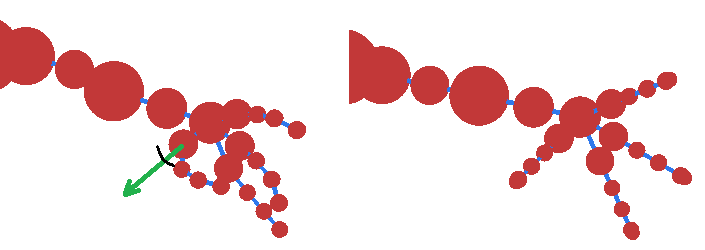
\includegraphics[width=\textwidth]{images/straightening2.png}
    \label{fig:straightening_ilu}
    \caption[Skeleton straightening]{Skeleton straightening; Left: input skeleton, green arrow represents the direction from connection nodes parents position to connection nodes position, black curve marks the distance between connection node and its child; Right: straightened skeleton}
\end{figure}

\subsection{Skinning matrices}
\paragraph{}
In final vertex placement we need to undo the rotations applied to the input skeleton during straightening. We have decided that the best solution is to use skinning, since it can be implemented on GPU and we wanted to move all post-processing on the GPU. Straightened skeleton represents bind pose for skinning purposes and the input skeleton represents reference pose. Now we can calculate skinning matrices required to transform bind pose to reference pose. Traditionally that would require to find the rotation between two corresponding nodes in respect to they parent. Rotating all child nodes in bind skeleton using the same rotation and propagate the rotation calculation to child nodes. But since we know precisely how bind pose was constructed, we can exploit this knowledge and avoid the rotation of child nodes. In fact we do not even need the bind skeleton itself.

\paragraph{}
This can be seen in Figure \ref{fig:DoF_estimation_ilu}. We want to calculate the rotation that would transform circle node to reference pose. We know that circle nodes parent square node is already in reference pose. We also know, that bind pose was constructed in such a way that all connection nodes childes are co-linear and preserve the distances between nodes. That means from squares reference pose we can calculate, where would be circle node, if we would apply on it the same transformation matrices as were applied to square node. The distance between square and circle node remains constant in both poses. And the direction at which the circle node would be is the same as the direction from triangle node to square node, which is marked as green arrow in Figure \ref{fig:DoF_estimation_ilu}. Now we only need to store the rotation between calculated circle node position, green circle in Figure \ref{fig:DoF_estimation_ilu} and its actual position red circle, with respect to its parent red square node.

\begin{figure}[h]
    \centering
    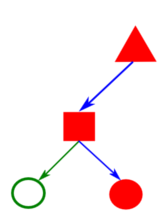
\includegraphics[height=6cm]{images/DoF_estimation.png}
    \label{fig:DoF_estimation_ilu}
    \caption[Rotation estimation from reference pose]{Rotation estimation from reference pose. Circle: node which rotation we want to estimate; Square: parent of circle node; Triangle: parent of square node; Blue arrows: edges in reference pose; Green circle: circle node position after applying squares skinning matrices; Green arrow: direction from square to green circle node;}
\end{figure}

\section{BNP generation}
\paragraph{}
For each branch node we calculate the direction from said branch node to each of its children and to its parent. Then we create rays, with origin in branch nodes position and direction corresponding to the direction calculated previously. These rays can be seen in Figure \ref{fig:bnp_gen_ilu} (a) as blue arrows. We calculate the intersection of each of these rays with a sphere associated with the branch node. We store each intersection in a set of intersection points. Now we triangulate the intersection points. Different algorithms can be used to achieve the same effect, but we have picked Delaunay triangulation in spherical domain, which was used in the original paper. The algorithm works like standard Delaunay triangulation, but the predicate deciding whatever newly inserted triangle would lie in the circle of an already existing triangle is replaced. The new predicate compares angle between the newly inserted triangles normal with normals of already existing triangles. Result of triangulation is shown in Figure \ref{fig:bnp_gen_ilu} (b) as the blue triangle. The generated polyhedron is now subdivided by inserting a point in the center of each face and in the middle edge. The vertex inserted in the center of each face is then connected with all vertices corresponding to the same face. So each triangle is subdivided into six smaller triangles. The newly inserted points are then projected onto the sphere associated with the node. The subdivision and projection is necessary, because otherwise polyhedrons that would be generated with co-planar, or nearly co-planar intersection points would have no volume or very little volume respectively. To project the newly inserted vertices onto the sphere, we once again use a ray. The origin of the ray is the position of each newly inserted vertex. The direction of the ray is mean normal of the faces that are connected with the vertex. This means that for the vertices in the center of each face the normal of the subdivided face is used. For vertices inserted in the middle of each edge the mean normal of faces corresponding to that edge is used. Final polyhedron is shown in Figure \ref{fig:bnp_gen_ilu} (c).

\begin{figure}[h]
    \centering
    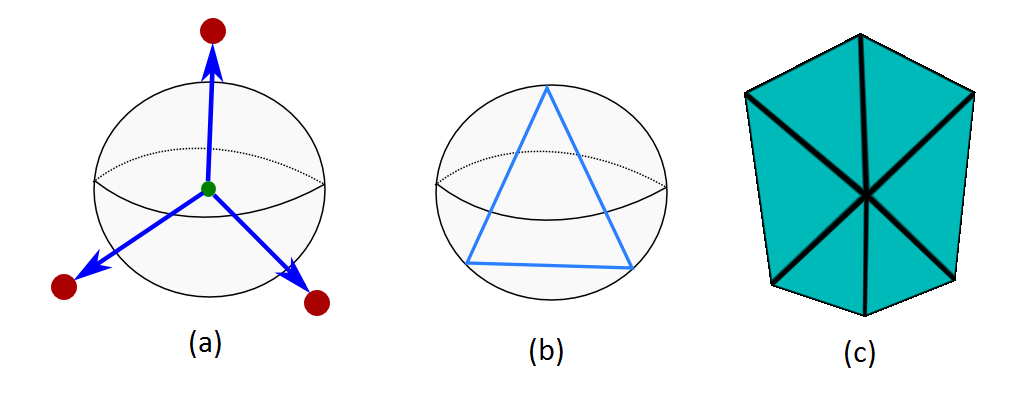
\includegraphics[width=\textwidth]{images/bnp_gen_ilu.png}
    \label{fig:bnp_gen_ilu}
    \caption[BNP generation process]{BNP generation process. (a) green is a branch node, blue arrows represent direction vectors of rays, red circles represent child nodes; (b) blue trinagle is the result of triangulation; (c) final subdivided BNP;}
\end{figure}

\paragraph{}
Triangulation of intersection vertices can sometimes create obtuse triangles. These are problematic, because when we insert the vertex in the middle of an obtuse triangle the one-rings of intersection vertices are not convex. That is if we would project them onto a plane defined by their principal axis and one of the vertices, the resulting polygon would not be convex. In Figure \ref{fig:obtus_tri_ilu} we can see on the left how a polyhedron looks when it is generated with obtuse triangles. Expected central vertex position is marked by red arrow, also expected edges are marked as yellow lines. This is not desirable, since it would cause problems during cyclic mesh generation. To remedy this situation we calculate the projection of the central vertex in a different manner. The origin of its ray is still vertex position. But we use a new direction vector. This vector is the normal of a triangle formed by the projected points that were inserted in the middle of each edge. The result can be seen in Figure \ref{fig:obtus_tri_ilu} on the right.

\begin{figure}[h]
    \centering
    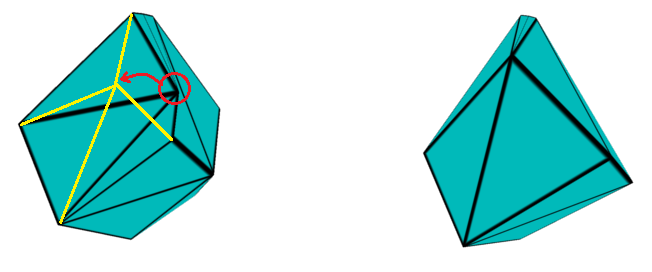
\includegraphics[height=6cm]{images/obtuse_triangle_fix_ilu.png}
    \label{fig:obtus_tri_ilu}
    \caption[Obtuse triangle problem]{Obtuse triangle problem. Left: polyhedron with obtuse triangle. Red arrow marks vertex expected position and yellow lines mark expected edges; Right: polyhedron after applying our fix;}
\end{figure}

\section{BNP refinement}
\paragraph{}
During the penultimate step of the algorithm, BNP joining, we want to connect two BNPs, with tube consisting solely from quadrilaterals. To ensure that we can use quadrilaterals only, we want intersection vertices connected via a path, to have the same number of nodes in their one-ring neighbourhood. We take the notion of Link Intersection Edge (LIE) from \cite{sqm}. A LIE is a set of edges that are between vertices of two intersection vertices one-ring neighbourhoods, as can be seen in Figure \ref{fig:refinement_ilu} (a). One LIE is represented with yellow colored edges and second LIE is represented with red colored edges. The refining of one BNP is a one-pass procedure.

\paragraph{Preprocessing}
We start the refining of a BNP by creating a map of LIEs corresponding to each intersection vertex. For each intersection vertex we store its corresponding LIEs, as well as the number of splits required by that vertex, to have the same valency as its corresponding intersection vertex. An intersection vertex can be connected with three types of vertices. Each type defines how much we can split LIEs corresponding to that intersection vertex.
\begin{itemize}
	\itemsep-0.25em 
	\item \textbf{Parents intersection vertex} - the number of splits is fixed. That is after spiting the valency of these two vertices must be exactly the same. This is necessary otherwise splits in child BNP could cause splits in parents BNP, which could result in infinite loops.
	\item \textbf{Branch node intersection vertex} - difference between valencies of the two vertices is calculated. If the number is negative, that is corresponding vertex has smaller valency, we prefer not to split LIEs corresponding the vertex any more. If the number is positive, that is corresponding vertex has higher valency, we split LIEs corresponding to the vertex so that the vertex has at least the same valency as its corresponding vertex.
	\item \textbf{Leaf node} - corresponding LIEs can be split as much has needed.
\end{itemize}

\begin{figure}[h]
    \centering
    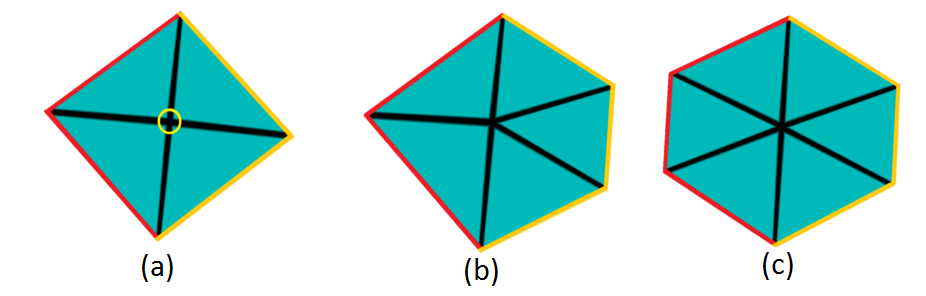
\includegraphics[width=\textwidth]{images/refinement_ilu.png}
    \label{fig:refinement_ilu}
    \caption[BNP refinement]{BNP refinement. Yellow edges represent Link Intersection Edge (LIE) corresponding to second intersection edge of the BNP. Red edges represent LIE corresponding to third intersection edge. Yellow circle marks the first intersection vertex. BNP before subdivision (a); BNP after one subdivision and one smoothing step (b); Final BNP after two subdivisions and two smoothing steps (c);}
\end{figure}

\paragraph{Subdivision}
We loop through all intersection vertices, starting with the intersection vertex connected with parents BNP and continuing with the rest. In each cycle, we split LIEs corresponding to current intersection vertex, until the valency of the intersection vertex is equal to its required number of splits. Every time we want to split a LIE we heuristically select the best, based on two filters. The first filter is the splitting required by the other intersection vertex belonging to the same LIE. If two or more LIEs require the same number of splits, we use a second filter. This filter picks the LIE that was split the least. When we are splitting a LIE, we always split a representative edge, which is the first edge of the LIE. Because of that we need to apply a smoothing scheme to roughly equalize the lengths of edges in a LIE. 

\paragraph{}
The whole process can be seen in Figure \ref{fig:refinement_ilu}. In Figure \ref{fig:refinement_ilu} (a) the yellow circle marks an intersection vertex that needs to be split twice. Yellow edges represent a LIE corresponding to second intersection vertex and red edges represent a LIE corresponding to third intersection vertex. Both LIEs have the same need to be split and non of them was split previously. For the first split the yellow LIE is selected, subdivided once and smoothed. The result of the first split is shown in Figure \ref{fig:refinement_ilu} (b). For the second split the need of both LIEs is still the same. But yellow LIE was already split, so this time the red LIE is selected, subdivided and smoothed. Final refined BNP is shown in Figure \ref{fig:refinement_ilu} (c).

\subsection{Smoothing}
\paragraph{}
Since we always split only one representative edge of a LIE, we are applying a smoothing scheme, to equalize the length of edges in a subdivided LIE. The smoothing is very important because directly on it depends the quality of the generated mesh. Ideally the length of each edge in a smoothed LIE would be equal. However since smoothing is applied after every subdivision, the smoothing algorithm should to be reasonably fast. We propose four smoothing schemes. These smoothing schemes are illustrated in Figure \ref{fig:smoothing_ilu}, where the polyhedron from Figure \ref{fig:refinement_ilu} is subdivided twice and then smoothed with various smoothing schemes.

\paragraph{Averaging smoothing}
New position for each vertex in a LIE is calculated by averaging one-ring neighbourhood corresponding to the vertex. We start with the last vertex of a LIE, that is the vertex on the last edge of a LIE and move towards the first vertex. We move each vertex, except the first and the last vertices, to the barycentre of its one-ring neighbourhood and project them back onto the sphere corresponding to BNPs node. The resulting smoothed polyhedron is shown in Figure \ref{fig:smoothing_ilu} (a). This approach is iterative and would need several iteration to achieve global optimum, however we have found that one iteration is enough for our needs.

\paragraph{Quaternion smoothing}
For each LIE we calculate a quaternion representing the rotation from the first vertex of the LIE to the last vertex of the LIE. From each quaternion we extract its corresponding axis of rotation and angle of rotation. We smooth only points between the first and the last vertex, so the calculated axis of rotation and angle are constant. During each smoothing step, we first count the number of vertices in a LIE. Then we divide the angle of rotation by that number and form a new quaternion from already calculated axis of rotation and the newly calculated angle. For each vertex in a LIE between first and last we apply the rotation stored in the quaternion and update its position. This method produces LIEs, that lie on small circles of their corresponding sphere. The spacing between vertices is regular and thus its very suitable for our needs. The result of quaternion smoothing is shown in Figure \ref{fig:smoothing_ilu} (b).

\paragraph{Area weighted Laplacian}
For Laplacian smoothing we have adapted the algorithm described in \cite{laplac_phd}. The weights used for smoothing are based on the one-ring area of each vertex. We use one iteration of Laplacian smoothing and then project the new vertices back onto their corresponding sphere. The result is shown in Figure \ref{fig:smoothing_ilu} (c). The result is usable, since the edges have better distributed length, than without smoothing. But averaging and quaternion smoothing produce results of better quality.

\begin{figure}[h]
    \centering
    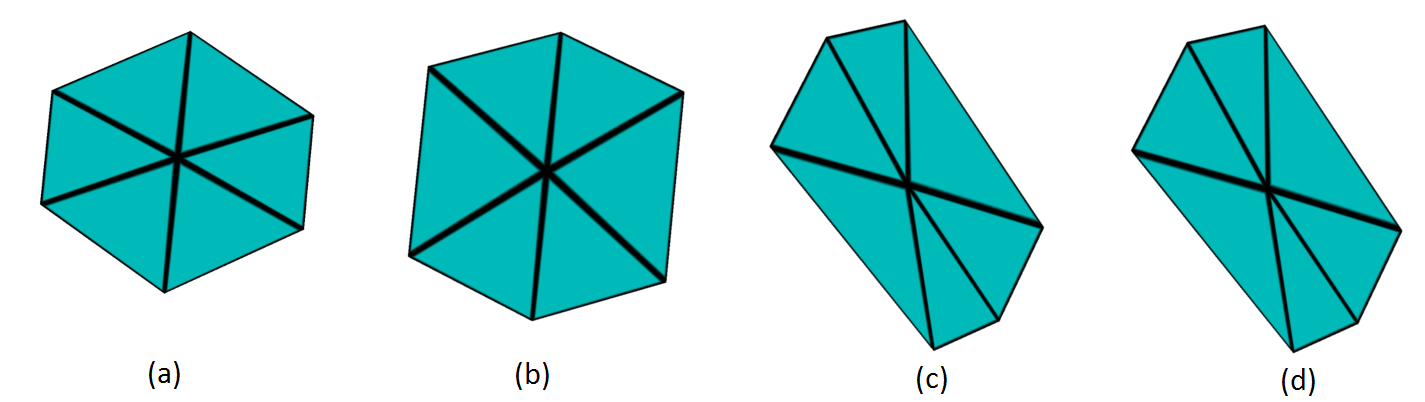
\includegraphics[width=\textwidth]{images/smoothing_ilu.png}
    \label{fig:smoothing_ilu}
    \caption[LIE smoothing schemes]{LIE smoothing schemes. Shows results after applying averaging smoothing (a); Quaternion smoothing (b); Area weighted Laplacian smoothing (c); and Valency weighted Laplacian smoothing (d);}
\end{figure}

\paragraph{Valency weighted Laplacian}
We use the same algorithm as for area weighted Laplacian, but we use different weights for vertices. The weights depend on the valency of each vertex. After Laplacian smoothing vertices are projected back onto their corresponding sphere. The result of this smoothing is very similar to area weighted Laplacian and is shown in Figure \ref{fig:smoothing_ilu} (d).

\section{BNP joining}